
\begin{abstract}
Failure attribution in LLM multi-agent systems—identifying the agent and step responsible for task failures—provides crucial clues for systems debugging but remains underexplored and labor-intensive. 
In this paper, we propose and formulate a new research area: \textbf{automated failure attribution} for LLM multi-agent systems.
To support this initiative, we introduce the \textbf{Who\&When} dataset, comprising extensive failure logs from 127 LLM multi-agent systems with fine-grained annotations linking failures to specific agents and decisive error steps.
Using the Who\&When, we develop and evaluate three automated failure attribution methods, summarizing their corresponding pros and cons. 
The best method achieves 53.5\% accuracy in identifying failure-responsible agents but only 14.2\% in pinpointing failure steps, with some methods performing below random. 
Even SOTA reasoning models, such as OpenAI o1 and DeepSeek R1, fail to achieve practical usability.
These results highlight the task's complexity and the need for further research in this area. Code and dataset are available in \href{https://github.com/mingyin1/Agents_Failure_Attribution}{the public repository}.
\end{abstract}


\section{Introduction}
\label{sec:intro} 
In recent years, the reframing Large Language Models (LLMs) as agents and built agentic multi-agent systems—composed of interactive, LLM-powered agents collaborating to achieve shared goals—has garnered significant attention~\citep{wu2023autogen, li2023camel, hong2023metagpt}. 
These purposefully designed agentic systems have demonstrated remarkable potential across various domains, including coding~\citep{hong2023metagpt}, scientific discovery~\citep{ghafarollahi2024sciagents}, and addressing complex real-world challenges~\citep{fourney2024magentic}.

Once constructed, these systems are typically refined through an iterative process when they fail in specific scenarios: evaluation against established benchmarks, followed by manual failure attribution and system refinement. 
This cycle repeats until the desired outcomes are achieved. 
Failure attribution—identifying the components of the system that directly lead to task failures—is a crucial step that serves as the foundation for guiding improvements. 
Despite its importance, this process is largely overlooked in mainstream research, which typically leaves it as a manual task requiring significant labor, such as analyzing complex historical logs and navigating the technical intricacies of the system. 
Moreover, mapping benchmark evaluation results to failure components is heavily dependent on domain expertise, imposing additional requirements on practitioners.
As systems grow in complexity, this challenge becomes increasingly difficult due to the growing number of components that must be considered when conducting failure attribution. 

\begin{figure}[!t]
\begin{center}
\centerline{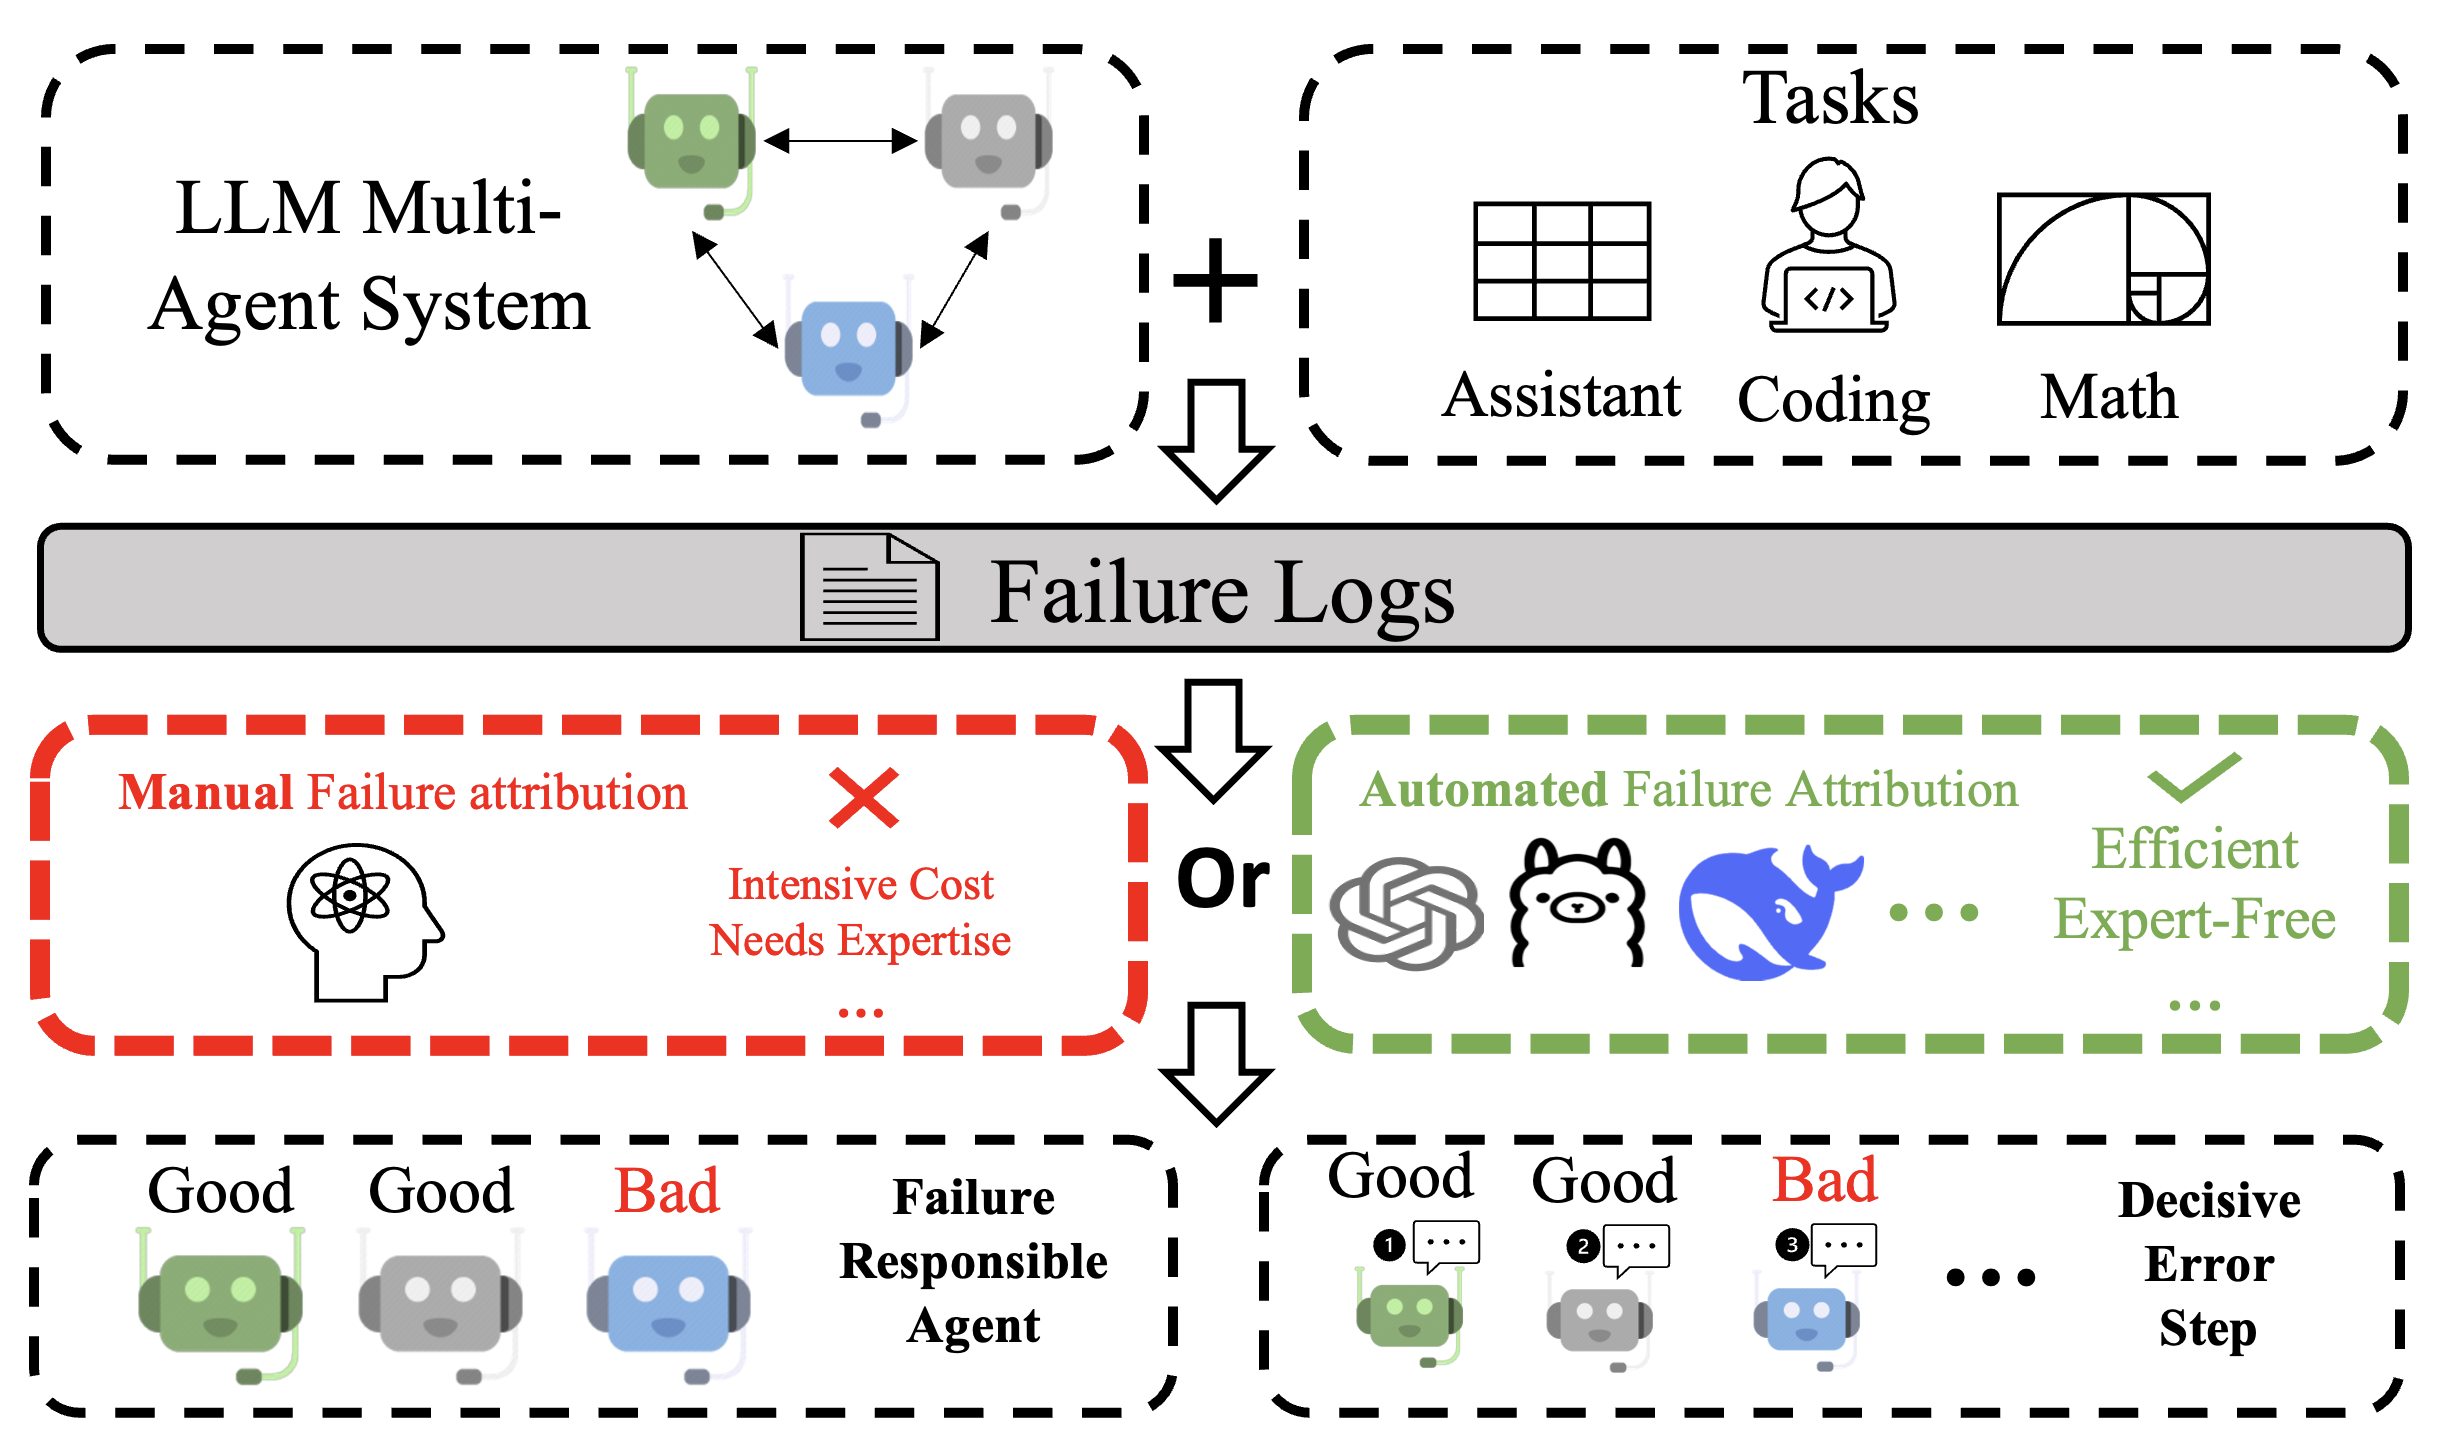
\includegraphics[width=1.0\columnwidth]{fig/overview.png}}
\caption{When developing LLMs-powered multi-agent systems, failure attribution—identifying system components responsible for task failures based on evaluation results—has received limited attention in existing research. This process is typically performed manually, demanding substantial labor and specialized expertise. In this study, we explore the potential for automating this process.}
\vspace{-30pt}
\label{fig:overview}
\end{center}
\end{figure}

Previous manual efforts involve a non-straightforward way to facilitate failure attribution in multi-agent systems: developing increasingly fine-grained benchmarks, with the hope that more metrics will enable quicker failure attribution~\citep{zhuge2024agent}.
For example, DevAI~\citep{zhuge2024agent} introduces a coding benchmark that incorporates diverse delivery requirements, offering a more nuanced evaluation compared to the widely used SWE-Bench~\citep{jimenez2023swe}, which focuses exclusively on final resolution rates. 
Despite these advancements, the process of failure attribution based on benchmark results remains a manual process, merely providing more metrics as reference points without fundamentally addressing the underlying challenges. 
With increasingly comprehensive benchmarks, a fundamental question remains unanswered: \textbf{which components of the agentic system require improvement?}

We argue that evaluation and failure attribution should be tightly integrated, adhering to the principle that ``evaluation is not an end in itself, but a means to improvement.''~\citep{scriven1991evaluation}
More research efforts should focus on bridging the substantial gap between evaluation results and failure attribution, which currently relies heavily on manual labor. 
Drawing inspiration from the LLM-as-a-judge paradigm~\citep{zheng2023judging, gu2024survey}, which leverages LLMs to replace human effort in evaluation, we propose to bridge the gap between evaluation and failure attribution by harnessing the comprehensive judgment capabilities of LLMs. 
Specifically, we propose and formulate a new research problem: \textbf{automated failure attributions} in LLM multi-agent systems. 
When failures occur under specific scenarios during evaluation, the goal is to automatically identify the components responsible for these failures without human intervention. 
We believe this research could serve as a substitute for manual failure attribution, enabling human resources to focus on improving system functionality rather than performing time-intensive diagnostics as shown in Figure~\ref{fig:overview}

To advance the research in this area, we introduce the \textbf{Who\&When} benchmark, comprising extensive failure logs annotated with fine-grained failure details for addressing real-world tasks, where these logs are collected from 127 LLMs-powered multi-agent systems.
This benchmark includes both algorithmically generated and hand-crafted multi-agent systems, encompassing a wide range of realistic scenarios.
Each failure log is accompanied by meticulous annotations, specifying the failure-responsible agent, the corresponding failure step, and the reasons for failure in plain language. 
The primary task involves pinpointing the agent most accountable for the failure and the exact step where the error occurred. 
Predicting the failure-responsible agent serves as a fundamental requirement for failure attribution, given that agents are the basic units of multi-agent systems. Extending this to the specific failure step prediction imposes a higher level of requirement, enabling more fine-grained failure attribution, such as uncovering the specific reasons behind failures, which can further facilitate targeted system refinements. We believe that Who\&When can serve as a foundational resource for driving progress in automated failure attribution research.

Additionally, we construct and evaluate several automated failure attribution approaches on the Who\&When. Our findings reveal the strengths and limitations of each method, as well as their performance across different conditions, including model variations, historical context lengths, and the presence or absence of query labels. The results underscore the complexity of using LLMs for failure analysis in multi-agent systems. For example, the best-performing method achieved only 8.77\% accuracy in identifying decisive error steps within the hand-crafted agentic system.